\documentclass[runningheads]{llncs}

\usepackage[T1]{fontenc}
% T1 fonts will be used to generate the final print and online PDFs,
% so please use T1 fonts in your manuscript whenever possible.
% Other font encondings may result in incorrect characters.

\usepackage{amsmath}

\usepackage{graphicx}

\usepackage{colortbl}
\usepackage{xcolor}

\usepackage{pifont}

\usepackage{booktabs}

\usepackage{tabularx}
\usepackage{multirow}

\usepackage{array}

\usepackage{marvosym}

\usepackage[hidelinks]{hyperref}
\hypersetup{
  colorlinks=true,
  linkcolor=red,
  citecolor=blue,
  urlcolor=blue,
  filecolor=blue,
  anchorcolor=blue
}

\usepackage{orcidlink}
\renewcommand{\orcidID}[1]{\,\orcidlink{#1}}

\newcolumntype{L}[1]{>{\raggedright\arraybackslash}p{#1}}
\newcolumntype{C}[1]{>{\centering\arraybackslash}m{#1}}
\newcolumntype{R}[1]{>{\raggedleft\arraybackslash}m{#1}}
\newcolumntype{Y}{>{\raggedright\arraybackslash}X}

\begin{document}

\title{Intra-Question Label Leakage in Knowledge Tracing with Multi-KC Questions: A Controlled Study on XES3G5M}
\titlerunning{Intra-Question Label Leakage in Knowledge Tracing}

% TODO: xác nhận danh sách, thứ tự và email với thầy/cô
\author{
Nhat-Anh Bui Nguyen\inst{1,4} \and
Anh-Kiet Vo\inst{1,4} \and
Thu Nguyen\inst{1,4}~\textsuperscript{(\Letter)}\orcidID{0000-0002-6577-0159} \and
Khoa Tan Vo\inst{1,4}\orcidID{0000-0002-5343-1686} \and
Phuc Nguyen\inst{2,4}\orcidID{0000-0002-6577-0159} \and
Tu-Anh Nguyen-Hoang\inst{3,4}\orcidID{0000-0001-9283-769X}
}
\authorrunning{N.-A. Bui Nguyen et al.}


\institute{Faculty of Information Science and Engineering, University of Information Technology, Ho Chi Minh City, Vietnam \and
Faculty of Information Systems, University of Economics and Law, Ho Chi Minh City, Vietnam \and
Information Security Laboratory, University of Information Technology, Ho Chi Minh City, Vietnam \and
Vietnam National University, Ho Chi Minh City, Vietnam
\\
\email{\{23520056,23520824\}@gm.uit.edu.vn, \{thunta,khoavt\}@uit.edu.vn, phucnq@uel.edu.vn, anhnht@uit.edu.vn}
\\[3pt]\textsuperscript{(\Letter)}\,Corresponding author: Thu Nguyen (thunta@uit.edu.vn)}


\maketitle

\begin{abstract}
ABSTRACT. % 150--250 từ; khung 7 câu ở mục 7.3 của nhận xét

\keywords{x \and x \and x \and x}
\end{abstract}

\section{Introduction}
Knowledge tracing (KT) predicts the probability that a student answers the next question correctly from their learning history. Most KT models work at the level of knowledge components (KCs), the skills that a question exercises, and a question can cover more than one of them: in XES3G5M~\cite{liu2023xes3g5m}, a large K-12 mathematics dataset with 5,549,635 interactions from about 18,066 students on 7,652 questions over 865 leaf-node KCs, each question is associated with 1.164 KCs on average.

The pyKT benchmark~\cite{liu2022pykt} treats such questions asymmetrically. 
In training, a multi-KC question is expanded into one token per KC, and every token carries the label of the question. 
In evaluation (all-in-one), every KC is predicted from the history before the question, and the KC predictions are then aggregated into a single question-level probability. 
Hence, when the second KC of a question is predicted in training, the first KC and the label to be predicted have already been read. 
A model can learn to copy the label of the preceding token instead of deriving it from the student's past performance, a shortcut that is useless at evaluation, where the label is never visible. 

Xiong et al.~\cite{xiong2016going} showed that DKT can exploit the repeated rows of multi-skill questions, and Badran and Preisach~\cite{DBLP:conf/csedu/BadranP25a,badran2026enhancing} identify label leakage in KC expansion and propose remedies (masked labels, fused updates, a question mask for attention). Still missing are a controlled measurement under the pyKT all-in-one protocol and a separation of what a remedy must change.

The remedy is a rule on the information available to each KC prediction, called Pre-Question Conditioning (PQC): (i) during training, the context of a prediction contains no information about the label of its own question; (ii) all KCs of a question are predicted from the same context as at evaluation, the history before the question. Condition (ii) implies (i), but some implementations meet (i) without (ii), so each step can be measured separately. PQC constrains what the model reads, not the architecture.
It is instantiated on DKT~\cite{piech2015deep} with five variants, and on simpleKT~\cite{DBLP:conf/iclr/0001L0H023} with a question mask on the attention.

On XES3G5M, standard DKT (3 seeds, 5 folds) is 0.098 AUC lower on the second and later KCs of multi-KC questions than on the first (0.7029 against 0.8008). PQC removes most of this gap and raises question-level AUC from 0.7841 to 0.7891 (+0.0050, 15 of 15 runs); on simpleKT (5 folds) it raises AUC by +0.0043 (5 of 5 runs). In both models the gain is concentrated in multi-KC questions (+0.032 and +0.024 AUC). On simpleKT the rule costs 0.0027 AUC on single-KC questions, concentrated in immediate repeats of the same question, which our segment convention hides from the model (Sect.~\ref{subsec:res-skt}).

Our contributions are:
\begin{enumerate}
  \item We measure intra-question label leakage under the pyKT all-in-one protocol: about 0.10 AUC is lost on the later KCs of multi-KC questions for DKT and about 0.13 for simpleKT.
  \item We state PQC, a two-condition rule that removes it without changing the architecture (+0.0050 AUC on DKT, +0.0043 on simpleKT, with better Brier score and lower ECE), and decompose its effect: (i) gives +0.0045, (ii) a further +0.0011, and the implementation is a second-order effect (at most 0.0006).
  \item We analyse the gain by question group, KC position and position in the student's sequence.
\end{enumerate}
The masked-label, fused-update and question-mask variants come from earlier work~\cite{DBLP:conf/csedu/BadranP25a,badran2026enhancing}. Our results concern one dataset and two backbones: DKT carries the main analysis (3 seeds, 5 folds), simpleKT has one seed (5 folds).

\section{Related Work}      \paragraph{KT models}
DKT~\cite{piech2015deep} reads the sequence of (KC, label) pairs with an LSTM. 
DKVMN~\cite{zhang2017dynamic} adds a key--value memory, SAKT~\cite{pandey2019self} replaces the recurrence by attention, AKT~\cite{ghosh2020context} adds monotonic attention with a Rasch-style question difficulty, and simpleKT~\cite{DBLP:conf/iclr/0001L0H023} uses standard attention with a question difficulty vector. 
Question-level models such as QIKT~\cite{chen2023improving} use one step per question, so they have no intra-question label leakage by construction, but they change the architecture and the input. 
Our rule targets KC-level models, which remain widely used and can be corrected without such a change; in pyKT's expanded sequences, recurrent and attention mechanisms read the earlier KC tokens of the same question, and we measure this only for DKT and simpleKT.
 
\paragraph{Multi-KC questions, label leakage and protocols.}
Xiong et al.~\cite{xiong2016going} observed that DKT benefits from repeated rows of multi-skill questions (average AUC 0.81 against 0.74 with one row per question on ASSISTments 2009--2010). 
Badran and Preisach~\cite{DBLP:conf/csedu/BadranP25a} name label leakage in KC expansion and propose a masked label for the KCs before the last one (DKT-ML), a fused update with one step per question (DKT-Fuse) and a question mask in attention (AKT-QM), the journal extension~\cite{badran2026enhancing} adds further variants (DKT-ML+, SAKT-ML, AKT-Fuse). 
They also propose an autoregressive variant (DKT-AD) and report that leakage grows with the number of KCs per question; in their KTbench evaluation the leaking baselines are tested all-in-one and the leak-free variants one-by-one. 
pyKT~\cite{liu2022pykt} standardizes KT evaluation (expanded training, all-in-one late fusion at test time), which makes numbers comparable but leaves training and evaluation different in what the model can read. 
We keep the pyKT protocol on XES3G5M~\cite{liu2023xes3g5m}, which provides pyKT baselines.
 
\paragraph{Position of this work.}
The variants of Badran and Preisach~\cite{badran2026enhancing} are taken here as design points, not claimed as our own. This work differs in three ways. First, the remedy is split into two conditions, and their effects are measured separately. Second, every model, leak-free variants included, is evaluated with the same pyKT all-in-one protocol on XES3G5M, with 3 seeds, 5 folds and a bootstrap over students. Third, the remedy is stated as a rule on the context of each prediction, which applies to both a recurrent and an attention backbone while keeping the per-KC loss. We do not propose a new architecture or aim to outperform AKT, simpleKT or QIKT.
\section{Problem Formulation}   \subsection{Notation}
The goal of the knowledge tracing problem is to predict the probability that a student will correctly answer any given question $q^*$ in the future, based on that student's past history of learning interactions. Let $\mathcal{Q}$ be the set of questions and $\mathcal{C}$ be the set of knowledge components (KCs). The history of student learning interactions is a sequence of $T$ question attempts $\mathcal{S} = \big((q_t, C_t, r_t)\big)_{t=1}^{T}$, where $q_t \in \mathcal{Q}$ is the question answered at step $t$, $C_t \subseteq \mathcal{C}$ is the set of KCs covered by $q_t$, $m_t = |C_t|$, and $r_t \in \{0, 1\}$ represents the accuracy of the response; $r_t = 0$ indicates an incorrect response, while $r_t = 1$ indicates a correct response.
The KCs of question $q_t$ form an ordered set $C_t = \{c_{t,1}, \dots, c_{t,m_t}\}$. A question with $m_t > 1$ is a \emph{multi-knowledge-component (multi-KC) question}. Importantly, $r_t$ is a single label for the whole question, not one label per KC.
Given the history $\mathcal{S}$, the model predicts the probability that the student answers the next question $q_{T+1}$ correctly, i.e.,
\begin{equation}
    P\big(r_{T+1} = 1 \mid q_{T+1}, C_{T+1}, \mathcal{S}\big).
\end{equation}

\subsection{The pyKT Protocol: Expanded Training and All-in-One Evaluation}

We follow the pyKT benchmark protocol~\cite{liu2022pykt}, which trains models
at the KC level but evaluates them at the question level.

\textbf{Training.} Each question in set $S$ for which $m_t > 1$ (i.e., a question associated with multiple knowledge components) is expanded into a sequence of $m_t$ interactions: $(q_t, c_{t,1}, r_t), \dots, (q_t, c_{t,m_t}, r_t)$, where the response $r_t$ for each of these expanded interactions is derived from the original question itself. Models are trained on expanded sequences.

\textbf{Evaluation.} Ground truth is observed only at the question level
(one label $r_t$ per question, not per KC), so pyKT scores models on questions.
Each KC of $q_t$ is predicted independently, using only the history before
$q_t$, so that no KC prediction has access to $r_t$ through other KCs of the
same question. The KC-level predictions are then aggregated into a single
question-level prediction by late fusion; in this work we use mean fusion.

\subsection{Intra-Question Label Leakage}

Expanded training and all-in-one evaluation do not condition on the same information. In the expanded sequence, the $j$-th KC of question $q_t$ with $j > 1$ is predicted after the interactions $(q_t, c_{t,1}, r_t), \dots, (q_t, c_{t,j-1}, r_t)$ have been read, so the input already contains the label $r_t$ to be predicted. Only the first KC of each question is free of this leakage. At evaluation, all KCs of $q_t$ are predicted from the history before $q_t$, so $r_t$ is never visible. A model can therefore learn the shortcut of copying the label of the preceding token whenever it infers that the two KCs belong to the same question, instead of inferring $r_t$ from the student's history. This shortcut is useless at test time and degrades question-level performance. The effect grows with the number of KCs per question and with the correlation between co-occurring KCs~\cite{DBLP:conf/csedu/BadranP25a}.

\section{Training Rule: Pre-Question Conditioning}     Section 3.3 shows that expanded training allows a model to read $r_t$
before predicting the later KCs of $q_t$, whereas all-in-one evaluation never
does. Therefore, the training process should limit the input infomation for each KC prediction such that the KC being predicted does not utilize information from other KCs within the same question. The resulting rule is called Pre-Question Conditioning (PQC). PQC constrains what the model may read; it is not a new architecture. Sections 4.2 and 4.3 show how to enforce it in a recurrent and in an attention backbone, and Section 4.4 states which parts come from prior work.

\subsection{The Rule}
\label{sec:rule-def}

Let $S_{<t}$ be the interactions of questions $q_1,\dots,q_{t-1}$, and let
$\mathcal{X}_{t,j}$ be what the model reads, besides $(q_t,c_{t,j})$, when it
predicts the $j$-th KC of $q_t$. Expanded training uses
\begin{equation}
  \mathcal{X}^{\mathrm{exp}}_{t,j}
  = S_{<t} \cup \{(q_t,c_{t,i},r_t)\}_{i<j},
  \label{eq:ctx-exp}
\end{equation}
while all-in-one evaluation uses
\begin{equation}
  \mathcal{X}^{\mathrm{eval}}_{t,j} = S_{<t}.
  \label{eq:ctx-eval}
\end{equation}
PQC requires, for every question $q_t$ and every $j \le m_t$:
\begin{enumerate}
  \item[(i)] During training, the label of a sentence is not included in the state used to predict the KC of that same question: $\mathcal{X}_{t,j}$ must not contain information
        $r_t$.
  \item[(ii)] All KCs of a question are predicted from the student’s state before that question, in line with the all-in-one protocol used for evaluation: all KCs of $q_t$ are predicted from
        the same context, the history before $q_t$, as in
        Eq.~\eqref{eq:ctx-eval}.
\end{enumerate}
Requirement (ii) implies requirement (i), so the two are nested. Requirement (i) alone prevents the model from simply copying the label. Requirement (ii) goes further and makes the training context exactly the same as the evaluation context. The two are stated separately because some implementations meet (i) but not (ii) (DKT-ML below), which makes it possible to measure the contribution of each step.
Under PQC we train with the per-KC binary cross-entropy
\begin{equation}
  \mathcal{L} = -\sum_{t}\sum_{j=1}^{m_t}
  \Big[ r_t \log \hat p_{t,j} + (1-r_t)\log(1-\hat p_{t,j}) \Big],
  \qquad
  \hat p_{t,j} = P\big(r_t = 1 \mid q_t, c_{t,j}, \mathcal{X}_{t,j}\big),
  \label{eq:loss}
\end{equation}
and evaluate exactly as in Section 3.2 (independent KC predictions, mean fusion).
Because $r_t$ is given to the model only after all $m_t$ predictions for $q_t$
have been made, the model cannot copy the preceding label. If every question has
a single KC, the rule changes nothing. It matters for training only when a
question has multiple KCs, either through its own rows or through the state it
leaves for later questions..

\subsection{Instantiation on Deep Knowledge Tracing}
Deep Knownledge Tracing (DKT) [cite] reads a sequence of tuple $(c, r)$, where $c$ is a KC and $r$ is the response to the question associated with KC $c$. Following Section 3.2, a question $q_t$ is expanded into a sequence of tuple ${(c_{t,1}, r_t), (c_{t,2}, r_t), ..., (c_{t, m_t}, r_t)}$. Let $h_{t, j}$ be LSTM state after reading $j$-th token of $q_t$, with $h_{t, 0} = h_{t-1, m_{t-1}}$ the state left by the previous question. Each tuple $(c_{t,j}, r_t)$ is encoded as a vector $\mathbf{x}_{t,j} \in \mathbb{R}^{d}$ and
\begin{equation}
  \mathbf{h}_{t,j} = \mathrm{LSTM}\big(\mathbf{x}_{t,j},\, \mathbf{h}_{t,j-1}\big), \qquad
  \mathbf{y}_{t,j} = \sigma\big(\mathbf{W}\mathbf{h}_{t,j} + \mathbf{b}\big).
\end{equation}

\paragraph{DKT (baseline)} Every token carries the true label and the next token is predicted from the previous one:
\begin{equation}
  \hat p_{t,j}=y_{t,j-1}[c_{t,j}],\qquad X_{t,j}=S_{<t}\cup\{(c_{t,i},r_t)\}_{i<j}.
\end{equation}
For $j>1$ the state has already read $r_t$, so neither (i) nor (ii) holds. This is the leakage of Section 3.3.

\paragraph{DKT-ML [cite].} The prediction rule is unchanged, but the label is hidden on every token except the last one of the question:
$$\rho_{t,j}=\begin{cases}MASK & j<m_t\\ r_t & j=m_t\end{cases}\qquad X_{t,j}=S_{<t}\cup\{(c_{t,i},\bot)\}_{i<j}.$$
Here $MASK$ is a mask symbol with its own input channel. Since $r_t$ is revealed only after the last KC, (i) holds. However, $c_{t,j}$ is still predicted after reading $c_{t,1},\dots,c_{t,j-1}$, so the context differs from evaluation and (ii) does not hold.

\paragraph{DKT-C (PQC, ours).} Tokens keep the true label, $\rho_{t,j}=r_t$, and are still read sequentially, but every KC of $q_t$ is predicted from the state before the question:
$$\hat p_{t,j}=y_{t-1,m_{t-1}}[c_{t,j}]=\sigma\!\big(Wh_{t,0}+b\big)[c_{t,j}],\qquad X_{t,j}=S_{<t}.$$
Neither $r_t$ nor the other KCs of $q_t$ is visible to the prediction of $c_{t,j}$, so (ii), and therefore (i), holds. The tokens of $q_t$ still pass through the LSTM, but they only update the state used for $q_{t+1}$.

\paragraph{DKT-ML-C.} This variant combines both changes: the labels are masked as in DKT-ML, $\rho_{t,j}=MASK$ for $j<m_t$, and every KC is predicted from $h_{t,0}$ as in DKT-C. The prediction context is the same as DKT-C, so (ii) holds. The two differ only in what the state stores for later questions: DKT-C keeps $r_t$ on every KC token, DKT-ML-C only on the last one.

\paragraph{DKT-Fuse.}
Instead of $m_t$ tokens, question $q_t$ is represented by a single token, obtained
by averaging the encodings of its KC tokens, and the LSTM advances by one step per
question:
\begin{equation}
  \bar{\mathbf{x}}_t = \frac{1}{m_t}\sum_{j=1}^{m_t}\mathbf{x}_{t,j},
  \qquad
  \mathbf{h}_t = \mathrm{LSTM}\big(\bar{\mathbf{x}}_t,\, \mathbf{h}_{t-1}\big),
  \qquad
  \mathbf{y}_t = \sigma\big(\mathbf{W}\mathbf{h}_t + \mathbf{b}\big).
\end{equation}
Every KC of $q_t$ is predicted from the state before the question,
\begin{equation}
  \hat p_{t,j} = \mathbf{y}_{t-1}[c_{t,j}], \qquad X_{t,j} = S_{<t},
\end{equation}
so neither $r_t$ nor the other KCs of $q_t$ is visible, and (i) and (ii) hold. The
original fusion approach of Badran and Preisach~\cite{badran} averages the KC
predictions into a question-level probability,
$\hat p_t=\frac{1}{m_t}\sum_{j=1}^{m_t}\hat p_{t,j}$, and applies the binary
cross-entropy to $\hat p_t$. We do not average before the loss: each KC receives its
own term of Eq.~(4). Averaging is applied only at evaluation, as in
Section~3.2.

\subsection{Design Space and Provenance}
\label{sec:rule-origin}

Table~\ref{tab:design} lists all variants. The principle of hiding same-question
interactions in attention was introduced as AKT-QM by Badran and
Preisach~\cite{badran2025}; masked labels (DKT-ML) and fused updates
(DKT-Fuse) also come from their work~\cite{badran2025,badran2026}. We do not
claim these mechanisms. What we add is (a) stating the rule as two separate
requirements, (i) and (ii), (b) DKT-PQC-Seq, which satisfies both without extra
parameters, and DKT-PQC-Mask as an intermediate step, and (c) a controlled
measurement of each step, and of the rule on simpleKT, under the all-in-one
protocol of pyKT. Question-level models such as QIKT build one step per
question, so they have no intra-question leakage by construction and are not
the target of the rule. A further control, which changes only checkpoint
selection, is described in Sect.~\ref{sec:setup}.

\begin{table}[t]
  \caption{Design space of the training rule. $h_{t,j-1}$ is the state after the
  first $j-1$ KCs of $q_t$ and $h_{t-1}$ the state before $q_t$; (i) and (ii) are
  the requirements of Sect.~\ref{sec:rule-def}. Parameter counts are for our
  XES3G5M configuration.}
  \label{tab:design}
  \centering
  \scriptsize
  \setlength{\tabcolsep}{3pt}
  \begin{tabular}{@{}l p{2.6cm} p{1.5cm} c c r p{1.9cm}@{}}
    \hline
    Variant & Update by the KCs of $q_t$ & KC $j$ read from & (i) & (ii) & Params & Origin \\
    \hline
    DKT-Exp          & one step per KC, true label & $h_{t,j-1}$ & no  & no  & 588,465   & \cite{piech2015dkt,pykt} \\
    DKT-ML           & one step per KC, MASK except last & $h_{t,j-1}$ & yes & no  & 674,965   & \cite{badran2025} \\
    DKT-PQC-Mask     & as DKT-ML & $h_{t-1}$ & yes & yes & 674,965   & ours \\
    DKT-PQC-Seq      & one step per KC, true label & $h_{t-1}$ & yes & yes & 588,465   & ours \\
    DKT-Fuse         & one step per question & $h_{t-1}$ & yes & yes & 588,465   & \cite{badran2025}; per-KC loss ours \\
    simpleKT         & attention over rows $j<i$ & rows $j<i$ & no  & no  & 3,754,497 & \cite{liu2023simplekt,pykt} \\
    simpleKT-QM      & attention over rows $g_j<g_i$ & rows $g_j<g_i$ & yes & yes & 3,754,497 & AKT-QM principle~\cite{badran2025} \\
    \hline
  \end{tabular}
  % NOTE: regenerate the Params column by script from registry.csv; simpleKT-QM count to be confirmed (same as simpleKT).
\end{table}
\section{Experimental Setup} \subsection{Dataset, Models and Metrics}
\label{subsec:data}
We use XES3G5M~\cite{liu2023xes3g5m}, collected from an online mathematics platform for K-12 students in China: 5\,549\,635 interactions from 18\,066 students on 7\,652 questions, annotated with 865 leaf-node KCs.
A question has on average 1.1640 KCs, so multi-KC questions are a minority but not negligible: 12.5\% of the graded questions (those scored in the metrics, 137\,481 of 1\,099\,197) have more than one KC, and these are the cases where intra-question leakage can occur.
We evaluate on a fixed test set of 3\,613 students.
 
The five DKT variants of Table~\ref{tab:design} share the same hyperparameters and are trained with 3 seeds (42--44) $\times$ 5 folds, i.e.\ 15 runs per variant. 
We also run the pyKT default configuration with 5 folds and seed 42 (5 runs per model) for DKT, simpleKT, simpleKT-PQC, AKT and QIKT; simpleKT-PQC differs from simpleKT only by the mask of Eq.~\eqref{eq:skt-pqc}, and QIKT (one step per question) is a question-level reference. 
No hyperparameter was tuned. We report mean and sd over runs.
 
All models are evaluated with the all-in-one protocol of Section~\ref{subsec:pyKT-protocol}, and all metrics are computed at the question level, with one probability $\hat p_t$ (mean late fusion) and one label $y_t=r_t$ per question: \textbf{AUC} (main metric); \textbf{Brier} $\frac1N\sum_t(\hat p_t-y_t)^2$; \textbf{ECE} with 10 equal-width bins; and \textbf{AUPRC-wrong}, the area under the precision--recall curve with the incorrect response as the positive class and $1-\hat p_t$ as score. 
Higher is better for AUC and AUPRC-wrong, lower for Brier and ECE.
 
\paragraph{Implementation.}
We use pyKT (commit \texttt{eec087e}, with a question-mask option for simpleKT-PQC and a device fix for QIKT) on one NVIDIA T4 GPU (Kaggle); the checkpoint is the epoch with the best KC-level validation AUC of pyKT, except for the leak-free selection control. All models are trained with Adam and early stopping on validation AUC (patience 10); other hyperparameters are the pyKT defaults. The DKT variants use pyKT's \texttt{is\_repeat} flag and do not merge repeated attempts; simpleKT-PQC does (Sect.~\ref{subsec:int-simpleKT}). The pre-registered check counted merged positions over all positions of the
test file, graded or not: 1.04\%, above the 1\% threshold set before the runs,
which is recorded as a deviation (0.79\% on the training file). The 0.95\% of
Sect.~\ref{subsec:int-simpleKT} is the same phenomenon counted on graded questions only.

\subsection{Statistical Testing}
\label{subsec:boot}
We use a paired bootstrap that resamples students, because the questions of one student are correlated.
For two runs $a$ and $b$ on the same fold and seed, we draw 1\,000 replicates and weight every question by the resampling weight of its student.
In each replicate we compute $\Delta=\mathrm{metric}(b)-\mathrm{metric}(a)$ for AUC, Brier score and ECE.
We report $\Delta$ on the full test set together with the 95\% percentile interval (CI) over the replicates. 
Each comparison yields 15 differences (5 for the pyKT runs), summarized by mean, minimum, maximum and the number of runs whose CI excludes 0. 
A difference is \emph{clear} if it has the same sign in all runs and its CI excludes 0 in at least 8 of 15 runs (3 of 5), a \emph{trend} if it has the same sign but the CI excludes 0 in fewer runs and \emph{not distinguishable} if the sign changes between runs. 
Only clear differences are set in bold. 
The comparisons follow Section~\ref{subsec:rule-origin}: the steps DKT $\to$ DKT-ML $\to$ DKT-ML-PQC $\to$ DKT-PQC (evaluated on the same questions, so their $\Delta$ values add up to DKT-PQC $-$ DKT), the implementations of PQC against DKT and each other, and simpleKT-PQC against simpleKT.
 
\paragraph{Mechanism analyses.}
To check the mechanism, we repeat the paired bootstrap on subsets of the test questions defined by two labels. The target label says whether the predicted question has a single KC or multiple KCs. The previous label says whether the question immediately before it has a single KC or multiple KCs, or is unknown; it is unknown when the predicted question is the first graded question of its student (3\,613 questions).
We cut the test set by the target label alone (2 subsets), by the previous label alone (3 subsets), and by both crossed ($2\times 3=6$ subsets), giving 11 subsets in total. Table~\ref{tab:strata} reports 9 of them; the two previous-only cuts for a single-KC or a multi-KC previous question are unions of crossed subsets and are omitted.
If leakage is the cause, the gain should concentrate where the predicted question has several KCs.

As a second diagnostic, we report the KC-level AUC separately for the first KC and for the second and later KCs of multi-KC questions. Under standard training only the later KCs can see $r_t$, so a leaking model should be worse on them. It is never used to rank models. 
 
\subsection{Sanity Checks for Leakage}
\label{subsec:sanity}
Five checks verify that label copying is the cause and that the PQC variants do not leak (fold 0, seed 42). The intervention test is run on DKT and DKT-PQC, the other checks on the five DKT variants. 
\emph{Global shuffle} permutes the training labels over the whole set (validation AUC should be about 0.5). 
\emph{Shuffle by question} permutes question-level labels and copies each to all KCs of its question: the history carries no signal, but a leaking model can exceed 0.5 by copying the preceding KC. 
We report the best KC-level validation AUC and the test Brier score (random-label models output almost constant probabilities). 
\emph{Overfitting}: each variant must fit 4 training sequences, so low scores under shuffling do not reflect an inability to learn. 
\emph{Intervention test}: in a trained model we flip the label of one random multi-KC question with a next question, in each of 32 training sequences (5 draws), and record the largest change of prediction on the KCs of that question (\texttt{inside}) and on the next question (\texttt{after}); without leakage $\texttt{inside}\le10^{-6}$, and $\texttt{after}>0$ shows the history is still used. 
\emph{Positive control}: standard DKT must be flagged as leaking and DKT-PQC must pass.
\section{Results}          DKT numbers are means over 15 runs (3 seeds $\times$ 5 folds); numbers for simpleKT, AKT, QIKT and the pyKT DKT are means over 5 runs (5 folds, seed 42).
Differences are ``clear'', ``trend'' or ``not distinguishable'' as in Section~\ref{subsec:boot}; only clear differences are in bold in Tables~\ref{tab:decomp} and~\ref{tab:strata}.

\subsection{Main Results and Calibration}
\label{subsec:res-main}

% ===== TABLE 2 =====
\begin{table}[tbp]
  \caption{Main results on XES3G5M (mean over runs; $\pm$ is the sd over runs; DKT variants 15 runs, other models 5 runs). ACC uses a threshold of 0.5 and is not tested. Paired tests: Table~\ref{tab:decomp} (DKT) and Sect.~\ref{subsec:res-skt} (simpleKT). ``Ref.\ AUC'': value published for the pyKT model on XES3G5M.}
  \label{tab:main}
  \centering
  \scriptsize
  \setlength{\tabcolsep}{3pt}
  \resizebox{\textwidth}{!}{%
    \begin{tabular}{@{}lrllllrl@{}}
\toprule
Model & Runs & AUC & ACC & Brier & ECE & Params & Ref.\ AUC \\
\midrule
DKT & 15 & 0.7841 $\pm$ 0.0002 & 0.8172 & 0.1319 & 0.0111 $\pm$ 0.0015 & 588,465 & -- \\
DKT, leak-free selection & 15 & 0.7840 $\pm$ 0.0002 & 0.8172 & 0.1319 & 0.0111 $\pm$ 0.0015 & 588,465 & -- \\
DKT-ML & 15 & 0.7886 $\pm$ 0.0002 & 0.8189 & 0.1305 & 0.0056 $\pm$ 0.0022 & 674,965 & -- \\
DKT-ML-PQC & 15 & 0.7897 $\pm$ 0.0002 & 0.8192 & 0.1303 & 0.0047 $\pm$ 0.0014 & 674,965 & -- \\
DKT-PQC & 15 & 0.7891 $\pm$ 0.0002 & 0.8191 & 0.1304 & 0.0047 $\pm$ 0.0018 & 588,465 & -- \\
DKT-Fuse & 15 & 0.7894 $\pm$ 0.0001 & 0.8193 & 0.1303 & 0.0041 $\pm$ 0.0014 & 588,465 & -- \\
\midrule
DKT (pyKT) & 5 & 0.7834 $\pm$ 0.0001 & 0.8165 & 0.1322 & 0.0120 $\pm$ 0.0045 & 841,465 & 0.7852 \\
AKT (pyKT) & 5 & 0.8162 $\pm$ 0.0008 & 0.8261 & 0.1243 & 0.0172 $\pm$ 0.0014 & 6,824,518 & 0.8207 \\
QIKT (pyKT) & 5 & 0.8206 $\pm$ 0.0001 & 0.8294 & 0.1222 & 0.0076 $\pm$ 0.0074 & 13,290,684 & 0.8222 \\
\midrule
simpleKT (pyKT) & 5 & 0.8121 $\pm$ 0.0004 & 0.8235 & 0.1258 & 0.0191 $\pm$ 0.0017 & 3,754,497 & 0.8163 \\
simpleKT-PQC & 5 & 0.8164 $\pm$ 0.0004 & 0.8269 & 0.1238 & 0.0081 $\pm$ 0.0024 & 3,754,497 & -- \\
\bottomrule
\end{tabular}
%
  }
\end{table}

Table~\ref{tab:main} compares the models. The three PQC implementations of DKT reach an AUC of 0.7891--0.7897 against 0.7841 for standard DKT, and DKT-ML, which only removes the label from the context, lies in between (0.7886).
The ordering is the same for all three seeds, and the standard deviation over 15 runs (0.0001--0.0002) is about 25 times smaller than the gap between DKT-PQC and DKT.
DKT-PQC and DKT-Fuse add no parameters, so the gain does not come from model size; DKT-ML and DKT-ML-PQC add 86\,500 (+14.7\%) and are not better.
On simpleKT, the mask raises AUC by 0.0043 (0.0039--0.0050) and ACC from 0.8235 to 0.8269; AUC, Brier and ECE are clear in 5 of 5 runs.

PQC is not meant to close the gap between backbones: our best DKT variant is 0.022--0.027 below the pyKT simpleKT and AKT, while simpleKT-PQC is at the level of the pyKT AKT (0.8164 against 0.8162; no paired test) and 0.0042 below QIKT. Our pyKT runs are 0.0016--0.0045 below the published values (Table~\ref{tab:main}), so comparison with them is only indicative.

\paragraph{Calibration.}
The gain is not limited to ranking: ECE falls from 0.0111 to 0.0041--0.0047 and Brier from 0.1319 to 0.1303--0.1304.
The DKT variants with PQC are better calibrated than simpleKT (ECE 0.0191) and AKT (0.0172), although these have a higher AUC. On simpleKT the mask lowers ECE to 0.0081, close to QIKT (0.0076).

\subsection{Decomposition and Implementations}
\label{subsec:res-decomp}

% ===== TABLE 3 =====
\begin{table}[tbp]
  \caption{Paired bootstrap differences $b-a$ on DKT (AUC: mean [min; max] over 15 runs; CI: runs with CI above 0 / below 0; Brier and ECE: mean). Bold: clear difference.}
  \label{tab:decomp}
  \centering
  \scriptsize
  \setlength{\tabcolsep}{3pt}
  \resizebox{\textwidth}{!}{%
    \begin{tabular}{@{}l l c c c@{}}
\toprule
Comparison ($b-a$) & $\Delta$AUC [min; max] & CI & $\Delta$Brier & $\Delta$ECE \\
\midrule
DKT-ML $-$ DKT (i) & \textbf{+0.00448} [+0.00410; +0.00506] & 15 / 0 & \textbf{$-$0.00136} & \textbf{$-$0.00544} \\
DKT-ML-PQC $-$ DKT-ML (ii) & \textbf{+0.00109} [+0.00046; +0.00148] & 15 / 0 & \textbf{$-$0.00029} & $-$0.00092 \\
DKT-PQC $-$ DKT-ML-PQC (label) & \textbf{$-$0.00058} [$-$0.00121; $-$0.00005] & 0 / 10 & +0.00014 & $-$0.00005 \\
DKT-PQC $-$ DKT (total) & \textbf{+0.00499} [+0.00473; +0.00543] & 15 / 0 & \textbf{$-$0.00151} & \textbf{$-$0.00641} \\
\midrule
DKT-ML-PQC $-$ DKT & \textbf{+0.00557} [+0.00510; +0.00606] & 15 / 0 & \textbf{$-$0.00165} & \textbf{$-$0.00636} \\
DKT-Fuse $-$ DKT & \textbf{+0.00533} [+0.00483; +0.00568] & 15 / 0 & \textbf{$-$0.00161} & \textbf{$-$0.00696} \\
DKT-Fuse $-$ DKT-PQC & \textbf{+0.00034} [+0.00010; +0.00061] & 8 / 0 & \textbf{$-$0.00010} & $-$0.00055 \\
DKT-Fuse $-$ DKT-ML-PQC & $-$0.00024 [$-$0.00059; +0.00026] & 0 / 6 & +0.00004 & $-$0.00060 \\
\midrule
DKT-PQC $-$ DKT, leak-free selection & \textbf{+0.00506} [+0.00465; +0.00560] & 15 / 0 & \textbf{$-$0.00153} & \textbf{$-$0.00647} \\
DKT, leak-free selection $-$ DKT & $-$0.00007 [$-$0.00056; +0.00029] & 1 / 3 & +0.00002 & +0.00006 \\
\bottomrule
\end{tabular}
%
  }
\end{table}

Table~\ref{tab:decomp} separates the effect of the rule into the steps of Section~\ref{subsec:rule-def}.
Removing the label while keeping the sequential reading (condition (i), DKT $\to$ DKT-ML) adds 0.0045 AUC, and reading the state before the question (condition (ii), DKT-ML $\to$ DKT-ML-PQC) a further 0.0011; both are clear, with the interval excluding 0 in 15 of 15 runs.
Replacing MASK by the true label (DKT-ML-PQC $\to$ DKT-PQC) lowers AUC by 0.0006 (clear in sign, but small). The three steps add up exactly to the total $+0.0050$ in AUC, and likewise in Brier and ECE; most of the Brier and ECE gain comes from the first step.
The three implementations of the rule differ by at most 0.0006 AUC, about nine times less than the effect of the rule itself (DKT-Fuse is above DKT-PQC by 0.0003, interval excluding 0 in 8 of 15 runs; DKT-Fuse and DKT-ML-PQC cannot be distinguished).
We therefore do not rank them: what matters is that (i) and (ii) hold.
Finally, selecting the checkpoint of standard DKT with a leak-free criterion changes AUC by $-0.00007$ and the sign changes between runs (not distinguishable); against this variant DKT-PQC is still better by $+0.0051$ AUC, so the gain does not come from the way the checkpoint is chosen.

\subsection{Mechanism: Where the Gain Comes From}
\label{subsec:res-mech}

\paragraph{AUC by KC position.}
Figure~\ref{fig:kcpos} gives the KC-level AUC in multi-KC questions, for the first KC and for the second and later KCs.
Standard DKT is almost 0.10 AUC worse on the later KCs (0.7029) than on the first (0.8008; gap $-0.0978\pm0.0024$), and simpleKT and AKT show larger gaps ($-0.126$, $-0.135$).
This is what label copying predicts: under all-in-one evaluation the previous KC of the same question is not available, so the shortcut is useless exactly where it was learned.
The pyKT DKT shows the same drop ($-0.093$), so it does not come from our implementation.
DKT-ML, which still predicts KC $j$ after the earlier KCs of the question, is in between ($-0.048$).
With (ii) the gap is only about $-0.005$ (DKT variants) and $-0.0056$ (simpleKT-PQC), which we read as the baseline difficulty of later KCs.

\begin{figure}[tbp]
  \centering
  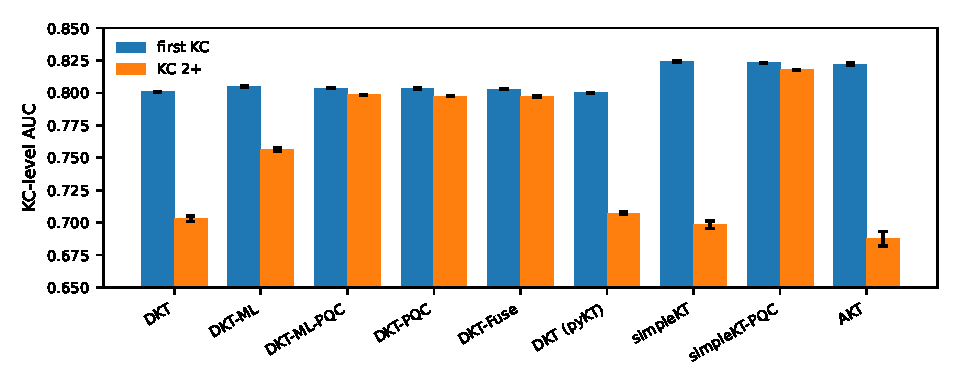
\includegraphics[width=\textwidth]{figures/fig2_kcpos.pdf}
  \caption{KC-level AUC in multi-KC questions, first KC against second and later KCs (mean over runs; error bars: sd over runs; DKT variants 15 runs, other models 5 runs). Diagnostic only, not used to rank models.}
  \label{fig:kcpos}
\end{figure}

\paragraph{AUC by question group.}
If leakage is the cause, the gain should be concentrated in multi-KC questions, and Table~\ref{tab:strata} shows that it is.
For DKT-PQC the AUC gain is $+0.0321$ on multi-KC targets (137\,481 questions) against $+0.0010$ on single-KC targets (961\,716); DKT-Fuse and DKT-ML-PQC behave the same way ($+0.0320$ and $+0.0328$ against $+0.0014$ and $+0.0016$).
For a fixed type of target the gain hardly depends on the previous question ($+0.0325$ and $+0.0314$ for multi-KC targets), so the target determines the gain, consistent with the leakage explanation.
On simpleKT the gain on multi-KC targets is similar ($+0.0242$, 5 of 5 folds), but on single-KC targets the mask is slightly worse ($-0.0027$, 5 of 5 folds); Sect.~\ref{subsec:res-skt} shows that this loss is concentrated in immediate repeats.

% ===== TABLE 4 (strata) =====
\begin{table}[tbp]
  \caption{Change in AUC by question group (target / previous question): DKT-PQC $-$ DKT (mean over 15 runs) and simpleKT-PQC $-$ simpleKT (mean over 5 runs). In parentheses: runs with a positive difference; then runs with CI above 0 / below 0. The last block (immediate repeats: the question ID equals that of the previous graded question) is given for simpleKT only, since DKT does not merge repeats (Sect.~\ref{subsec:int-simpleKT}). Bold: clear difference.}
  \label{tab:strata}
  \centering
  \scriptsize
  \setlength{\tabcolsep}{3pt}
  \resizebox{\textwidth}{!}{\begin{tabular}{@{}l r l@{}}
\toprule
Target / previous question & \#questions & DKT-PQC $-$ DKT (of 15) \\
\midrule
1 KC / all & 961\,716 & \textbf{+0.0010 (15; 15 / 0)} \\
multi-KC / all & 137\,481 & \textbf{+0.0321 (15; 15 / 0)} \\
\midrule
1 KC / 1 KC & 865\,139 & \textbf{+0.0011 (15; 15 / 0)} \\
1 KC / multi-KC & 93\,251 & +0.0006 (14; 2 / 0) \\
multi-KC / 1 KC & 93\,786 & \textbf{+0.0325 (15; 15 / 0)} \\
multi-KC / multi-KC & 43\,408 & \textbf{+0.0314 (15; 15 / 0)} \\
\midrule
1 KC / first graded question & 3\,326 & \textbf{$-$0.0067 (0; 0 / 9)} \\
multi-KC / first graded question & 287 & \textbf{+0.0452 (15; 12 / 0)} \\
all first graded questions & 3\,613 & +0.0001 (8; 0 / 0) \\
\bottomrule
\end{tabular}
}%
\end{table}

\subsection{Sanity Checks for Leakage}
\label{subsec:res-sanity}

Results of the checks of Section~\ref{subsec:sanity} (fold 0, seed 42):
\emph{Positive control:} flipping the label of a multi-KC question changes the prediction of its later KCs by up to 1.00 for standard DKT (flagged as leaking) and by 0 for DKT-PQC; the next question's prediction still changes in both, so the test is reliable.
\emph{Shuffled labels} (Table~\ref{tab:sanity}): with labels shuffled by question, only standard DKT learns from the shared label (best validation AUC 0.625); the four variants that satisfy (i) stay at 0.500--0.501. Test Brier separates them less cleanly (0.1631 for DKT and DKT-Fuse, 0.1625--0.1627 for the others), so we rely on validation AUC. With a global shuffle all variants fall to about 0.50, and all five fit 4 training sequences, so low scores under shuffling do not reflect an inability to learn.
\emph{Leak-free selection:} it gives the same test result as the default choice (AUC 0.7840 against 0.7841; Tables~\ref{tab:main} and~\ref{tab:decomp}), so the leakage is not an artifact of checkpoint selection.
These controls were run on DKT only; for simpleKT the evidence is the gap between first and later KCs and its removal by the mask (Figure~\ref{fig:kcpos}).

\subsection{First Graded Question of Each Student}
\label{subsec:res-first}

The gain is not uniform.
For the 3\,326 single-KC questions that are the first graded question of a student (0.3\% of the test questions), DKT-PQC is 0.0067 \emph{below} DKT: the difference is negative in all 15 runs and its interval excludes 0 in 9 (clear; Table~\ref{tab:strata}).
Over all 3\,613 first graded questions, including the 287 multi-KC ones (where DKT-PQC is 0.0452 \emph{above} DKT), the difference is $+0.0001$ and changes sign between runs, so this small group does not contradict the overall gain; we have not tested why standard DKT is better on it.
On simpleKT the mask is clearly better on the first graded questions as a whole ($+0.0087$, 5 of 5 folds; Table~\ref{tab:strata}): the gain on the 287 multi-KC ones ($+0.0399$) outweighs a small, not distinguishable difference on the single-KC ones ($-0.0012$).

\subsection{simpleKT-PQC versus simpleKT}
\label{subsec:res-skt}

Three criteria were fixed before the runs: (a) $\Delta$AUC $\ge 0.003$ and clear, (b) $\Delta$Brier $<0$ and clear, (c) a gap between later and first KCs within $\pm0.03$ in all five folds. All three hold. simpleKT-PQC raises AUC from 0.8121 to 0.8164 ($+0.0043$, from $+0.0039$ to $+0.0050$; CI excludes 0 in 5 of 5 folds), and lowers Brier by 0.0020 and ECE from 0.0191 to 0.0081, all clear (Table~\ref{tab:main}).
The gap between later and first KCs, $-0.1260\pm0.0032$ for simpleKT, becomes $-0.0056\pm0.0003$ (Figure~\ref{fig:kcpos}): the later KCs gain 0.1196 AUC and the first KC changes by $-0.0008$.
This is the pattern expected if the baseline copies the label of an earlier KC of its own question. Unlike DKT, simpleKT has no shuffle or intervention control, so the evidence agrees with label copying but does not isolate it.

\paragraph{Single-KC questions and immediate repeats.}
On single-KC questions the mask is slightly worse ($\Delta$AUC $=-0.0027$, from $-0.0033$ to $-0.0017$; negative in 5 of 5 folds, clear), while on multi-KC questions it is better ($+0.0242$; Table~\ref{tab:strata}).
The loss is concentrated in immediate repeats, i.e.\ a question attempted twice in a row. On the 9\,515 single-KC repeats ($0.99\%$ of the group) simpleKT-PQC is $0.1725$ AUC below simpleKT in all folds; on the 909 multi-KC repeats it is similar ($-0.1877$), so it does not depend on the number of KCs. Over all 10\,424 repeats (0.95\% of the test questions) $\Delta$AUC $=-0.1739$ and $\Delta$Brier $=+0.0616$ in 5 of 5 folds; $\Delta$ECE is $+0.0053$ with the same sign in all folds but a CI that includes 0 (trend).
On the other 99.05\% of the questions the gain is larger than overall ($\Delta$AUC $=+0.0062$ against $+0.0043$, 5 of 5 folds).
On single-KC questions that are not repeats the difference is $-0.0008$ (from $-0.0014$ to $+0.0001$); its sign changes between folds (not distinguishable by our rule), although the CI lies below 0 in 4 of 5 folds, so a small residual loss cannot be excluded.

A likely cause is our segment convention (Sect.~\ref{subsec:int-simpleKT}): consecutive attempts at the same question are merged, so the mask hides the attempt just before the one being predicted, which is legitimate history at test time and highly informative. In fold 0, 98.1\% of repeats are correct after a correct attempt, against 33.4\% after an incorrect one.
The rule does not require this merge, but we have not isolated its effect, and group AUCs are not additive.

\begin{table}[tbp]
  \caption{Sanity checks on fold 0 (seed 42), DKT variants. Intervention test: \texttt{inside} / \texttt{after}. Brier of a constant predictor: about 0.1626.}
  \label{tab:sanity}
  \centering
  \scriptsize
  \setlength{\tabcolsep}{3pt}
  \resizebox{\textwidth}{!}{%
    \begin{tabular}{@{}l c c c c c@{}}
  \toprule
  Check & DKT & DKT-PQC & DKT-ML & DKT-ML-PQC & DKT-Fuse \\
  \midrule
  Intervention, inside / after           & 1.00 / 0.80 (leaks) & 0 / 0.76 (pass) & -- & -- & -- \\
  Overfit 4 sequences, loss after 300 steps & 0.0013 & 0.0013 & 0.0013 & 0.0013 & 0.0014 \\
  Shuffle by question: best val.\ AUC    & 0.6250 & 0.5005 & 0.5004 & 0.5002 & 0.5008 \\
  Shuffle by question: test Brier        & 0.1631 & 0.1625 & 0.1626 & 0.1627 & 0.1631 \\
  Global shuffle: best val.\ AUC         & 0.5010 & 0.5007 & 0.5011 & 0.5012 & 0.5009 \\
  Global shuffle: test Brier             & 0.1630 & 0.1630 & 0.1627 & 0.1628 & 0.1629 \\
  \bottomrule
\end{tabular}%%
  }
\end{table}
\section{Discussion and Limitations} \paragraph{Mechanism.}
On DKT, three independent pieces of evidence point to label copying: the gap between first and later KCs (Fig.~\ref{fig:kcpos}), the shuffle-by-question control (0.625 against 0.500--0.501) and the intervention test (1.00 against 0). On simpleKT only the gap is available, so the evidence is indirect.

\paragraph{Validation in pyKT.}
The KC-level validation AUC of pyKT exceeds the test AUC by about 0.05 for every model that leaks: $+0.052$ for DKT and for the pyKT DKT, $+0.046$ for AKT and $+0.049$ for simpleKT. For the models that satisfy (ii) and for QIKT the difference is between $-0.003$ and $-0.002$. Selecting a model with the pyKT validation would therefore favour a leaking one. This agrees with the inflated validation reported by Badran and Preisach~\cite{DBLP:conf/csedu/BadranP25a}.

\paragraph{Size of the effect.}
The overall effect is small ($+0.005$ and $+0.004$ AUC) because only 12.5\% of the questions have several KCs.


\paragraph{Limitations.}
We use one dataset; simpleKT has one seed; the shuffle, intervention and leak-free-selection controls ran on DKT only; no hyperparameter was tuned, and our pyKT baselines are 0.0016--0.0045 AUC below published values. The segment convention of simpleKT-PQC is the likely cause of its loss of 0.17 AUC on immediate repeats and of most of its loss on single-KC questions (Sect.~\ref{subsec:res-skt}); we have not isolated its effect, and a small residual loss on single-KC questions that are not repeats ($-$0.0008) cannot be excluded. DKT-PQC is 0.0067 below DKT on single-KC first graded questions, which we have not explained. We do not rank the three implementations of the rule.
\section{Conclusion}       In pyKT, multi-KC questions are trained as one token per KC with the question's label but evaluated from the history before the question, so a model can learn to copy the label. Pre-Question Conditioning states what a KC prediction may read: no label of its own question, and the same context as at evaluation. On XES3G5M it raises AUC by $+0.0050$ on DKT and $+0.0043$ on simpleKT, lowers ECE, and gives $+0.032$ and $+0.024$ on multi-KC questions, while the implementation matters little (at most 0.0006). The evidence for copying is direct on DKT and indirect on simpleKT, where the segment convention also costs AUC on immediate repeats. Future work: exact question boundaries for attention backbones (to test whether they remove this loss), other datasets and models, and question-level validation.

\begin{credits}
\subsubsection{\ackname} This research is funded by \ldots

\subsubsection{\discintname}
% TODO: nếu nộp qua CMT, kiểm tra xem hội nghị có yêu cầu khai báo ở đây hay trong hệ thống nộp bài.
The authors have no competing interests to declare that are relevant to
the content of this article.
\end{credits}

\bibliographystyle{splncs04}
\bibliography{ref}

\end{document}